\documentclass[acmsmall,screen,nonacm]{acmart}

% ACM class controls page geometry, typography, headings, and float styling.
% Do not add geometry or manual spacing overrides.
\usepackage{microtype}
\usepackage{xurl}
\usepackage{float}

\setcopyright{none}
\settopmatter{printacmref=false, printccs=true, printfolios=true}

\title[Citation-Support Scoring Policies]{Citation-Support Scoring Policies Change System Gaps: A Controlled Reanalysis of Archived Human Annotations}

\author{Gorla Nitheesh Kumar}
\affiliation{%
  \department{Department of Information Technology}
  \institution{Indian Institute of Information Technology Allahabad}
  \city{Prayagraj}
  \state{Uttar Pradesh}
  \country{India}
}

\renewcommand{\shortauthors}{Kumar}

\begin{CCSXML}
<ccs2012>
 <concept>
  <concept_id>10010147.10010257</concept_id>
  <concept_desc>Computing methodologies~Natural language processing</concept_desc>
  <concept_significance>500</concept_significance>
 </concept>
 <concept>
  <concept_id>10002951.10003317</concept_id>
  <concept_desc>Information systems~Information retrieval</concept_desc>
  <concept_significance>300</concept_significance>
 </concept>
 <concept>
  <concept_id>10010147.10010257.10010293</concept_id>
  <concept_desc>Computing methodologies~Evaluation methodologies</concept_desc>
  <concept_significance>300</concept_significance>
 </concept>
</ccs2012>
\end{CCSXML}

\ccsdesc[500]{Computing methodologies~Natural language processing}
\ccsdesc[300]{Information systems~Information retrieval}
\ccsdesc[300]{Computing methodologies~Evaluation methodologies}

\fancypagestyle{numberonly}{%
  \fancyhf{}%
  \fancyhead[R]{\thepage}%
  \renewcommand{\headrulewidth}{0pt}%
  \renewcommand{\footrulewidth}{0pt}%
}
\begin{document}
\pagestyle{numberonly}
\setlength{\intextsep}{12pt}
 \raggedbottom
\begin{abstract}
Under two policies involving citation support, we rescore the fixed generative queries and archived human annotations for a piece of text. C0 - Credit for possibly qualifying partial citations for statements where evidence is combined together. C1 – Individual Full Support. After explicit adaptation of Liu et al.'s protocol, a four-system collection of 353 common queries was created, each of which has been successfully linked with a judgment, and the query weights are equal. For Bing Chat, Neeva, Perplexity and You, the reduction in precision is 0.826 percentage, 2.111 percentage, 3.753percentage and 1.220 percentage, respectively, across the different chat models. The largest absolute pairwise gap change is an increase of 2.927 points. Each and every group of six is ordered and bound with each other. The score losses are concentrated in a few responses and both tested alternatives to duplicate-handling and aggregation are found to have stability under ordering. Findings relate to a selected historical cohort.
\end{abstract}
\keywords{citation support, scoring sensitivity, reproducibility, human annotations, generative search}
\maketitle
\thispagestyle{numberonly}

\section{Introduction}
A real citation might give insufficient support for the quotation it is citing~\cite{liu2023,rashkin2023}. We recently reviewed some of the situations around citing fabricated, misattributed, and corrupted metadata, and this distinction reduces the list of such scenarios to a measurement question. The union of two sets A and B that both provide some support for the same statement may provide support for the whole statement. In that case, Liu et al. attribute it to partial sources qualifying the answer~\cite{liu2023}. The measured separation may vary between systems, depending on how much they rely on this credit, and a change in the rule for this credit can change the measured separation for systems if they rely on this credit to different extents.

\textbf{Research questions.}RQ1 to examine the extent and extent of the loss of precision for each system. The main questions RQ2 was concerned with are on how much each of the 6 pairwise precision gaps changed. RQ3 checks exact ties and reversals. The answers, labels, denominators and question weights are held constant in the main comparison.

\section{Related Work}
ALCE separates citation correctness and coverage and performs automatic inference on the evaluation of support component~\cite{gao2023}. AIS provides support with respect to the identified sources, while BEGIN provides evaluation of attribution in dialogue~\cite{rashkin2023,begin}. Summarization studies look at faithfulness and other categories of factual errors~\cite{maynez, frank} and FActScore takes atomic facts as the summarization unit~\cite{factscore}. Consistency has also been explored in the context of classification, entailment or question-answering in earlier work and grounding in retrieval-augmented generation is studied in this work. The predictors (human judgments) in the present experiment are relevant and comparable to those of the policies, but are fixed and already obtained from archives.

FactCC, QAGS, QAFactEval, and SummaC illustrate different units and procedures for factual consistency~\cite{factcc,qags,qafacteval,summac}. RAGAs, ARES, and RAGTruth address grounding or hallucination in retrieval-augmented systems~\cite{ragas,ares,ragtruth}. SummEval and TRUE motivate examining behavior below aggregate scores~\cite{summeval,true}. Annotation agreement, human-evaluation reporting, and dataset documentation inform interpretation of inherited judgments~\cite{agreement,howcroft,datastatements}. Work on repeatability and explicit metric configuration motivates documenting cohort and scoring choices~\cite{belz,post}.

\section{Data and Cohort}
We use the 17,520,509-byte archive \texttt{human\_evaluation\_annotations.jsonl} from Liu et al.'s companion repository~\cite{archive}, pinned to commit \texttt{2c6b485ae1c2}. It contains historical Bing Chat, Neeva, Perplexity, and You responses to 1,450 distinct query strings. The validation report records the SHA-256 fingerprint. Table~\ref{tab:structure} summarizes the raw archive.
\begin{table}[!htbp]
\centering\small
\caption{Independently checked archive structure. Counts precede exclusions.}
\begin{tabular}{lr}\toprule
Quantity & Count\\\midrule
Annotation rows & 5,528\\
Distinct response IDs & 5,457\\
Repeated-ID groups & 69\\
Excess structurally identical records & 47\\
Repeated groups with distinct records & 24\\
Citation objects & 15,828\\
Statement--marker entries & 15,169\\
Rows with unequal object/entry counts & 335\\
Zero-citation rows & 892\\
Null collective judgments & 9,075\\\bottomrule
\end{tabular}
\label{tab:structure}
\end{table}

\subsection{Original baseline and adaptation}
The published response-level precision is
\begin{equation}
 P_0=(T_{fs}+T_{ps})/N_{\mathrm{paper}}.
\end{equation}
Here $T_{fs}$ counts full-support citations, $T_{ps}$ counts qualifying partial-support citations, and $N_{\mathrm{paper}}$ is the published citation denominator. The archive leaves three conventions unresolved: counting occurrences, resolving repeated records, and aggregating zero-citation responses. In particular, 335 rows have different citation-object and statement--marker counts. We therefore use explicitly adapted controls C0 and C1. Exact reproduction of the published evaluation remains unresolved.

\subsection{Eligibility}
The main protocol adopts only one response record per retained query-system combination for each raw (no representation) response record. We validate offsets of citation characters; we can tell what parts of the unmodified version of a text need to be judged as cited and what parts do not; citations must be cited in exactly the same way as they were. Responses that contain unclear links, have lacked some of the necessary judgments, contain the wrong label or have no citations will not be eligible under either policy. The number of queries that are eligible for all four systems is 353, 1,412 is the number of responses and 4,382 is the number of mapped citation units in the intersection of all four systems in a query intersects response.353 queries, 1412 responses, and 4,382 mapped citation units is the numbers of queries, number of responses, and number of mapped citation units that the query intersects with the response in all four systems. The corresponding screen held 357 queries prior to the correspondence check. The proportions of the 12 source categories are changed and their cases are retained.

\section{Scoring and Validation}
Let $H_r$ be the number of mapped partial-support occurrences in reply $r$ and let $F_r$ be the number of mapped occurrences that provide full support on their own in $r$. These two policies have the same denominator.
\begin{equation}
 C0_r=\frac{F_r+H_r}{N_r},\qquad C1_r=\frac{F_r}{N_r}.
\end{equation}
Zero points will be awarded for inaccessible, unclear, and support–plus-refutation labels. Raw labels produced from the audit are preserved. If two or more C0s come together and provide a full supporting statement for a C0, then they are able to award a maximum of two half marks. In such an instance, C1 gives himself no partial credit for either of those references. When another citation is followed by a partial citation, then each one deserves only the other citation.

\subsection{Pairwise estimand}
For the common query set $Q$, each system has one retained answer per query. The variable $k$ indexes the control, and $P_{s,k}$ weights each query equally.
\begin{align}
 P_{s,k}&=|Q|^{-1}\sum_{q\in Q} Ck_{s,q},\\
 L_s&=P_{s,0}-P_{s,1},\\
 G_{ab,k}&=P_{a,k}-P_{b,k},\\
 D_{ab}&=G_{ab,1}-G_{ab,0}=L_b-L_a.
\end{align}
$L_s$ is the system's mean loss. $G_{ab,k}$ is the signed precision gap between systems $a$ and $b$. $D_{ab}>0$ means the signed advantage of $a$ over $b$ increases under C1. Response loss is $H_r/N_r$. Since $N_r>0$ and $H_r\geq0$, $C1_r\leq C0_r$ follows directly. The pooled sensitivity analysis weights each response by $N_r/\sum_{r'}N_{r'}$.

Exact rational arithmetics are used in all the calculations. Opposite nonzero at sign and gap sign is required for a strict reversal. A tie transition only needs an exact 0 under one policy. The selected archive is reported as quantities. Responses and answers to a single question may be dependent.

\subsection{Implementation and validation}
The python pipeline validates the input, reconcilates the annotations, creates a cohort, runs the score on both the policies, and aggregates the results. It ignores 0 denominators and/or nonuniform denominators. There are 18 unit tests that cover input malformed, input null, label handling, conditional credit, zero denominators, offsets, repeated markers and IDs, and repeated nulls. An arithmetic audit independently calculates the precise responses for each score label and the normalized gaps between labels for 4,346 scored record cases in 3 cohort variants. The audit will check calculations with the inherited annotations.

The clean workspace for Linux was run with Python 3.12.14, and Matplotlib 3.10.8. It took 9.755 seconds and achieved a max child resident memory of 87,524 KiB according to tests, validation, analyses, audits and figures. The standard Python libraries were used for scoring.

\section{Results}
\begin{table}[!htbp]
\centering\small
\caption{Primary results. Precision in percent; loss in percentage points. Affected counts are out of 353 queries per system.}
\begin{tabular}{lrrrr}\toprule
System & C0 & C1 & Loss & Affected\\\midrule
Bing Chat & 91.792 & 90.966 & 0.826 & 4 \\
Neeva & 69.187 & 67.076 & 2.111 & 16 \\
Perplexity & 76.295 & 72.542 & 3.753 & 27 \\
You & 62.367 & 61.147 & 1.220 & 6 \\
\bottomrule

\end{tabular}\label{tab:system}
\end{table}
\begin{table}[!htbp]\centering\scriptsize
\caption{Pairwise gaps and changes, all in percentage points. Pair orientation is fixed before scoring.}
\begin{tabular}{lrrr}\toprule
Pair ($a-b$) & $G_0$ & $G_1$ & $D$\\\midrule
Bing Chat--Neeva & 22.605 & 23.890 & +1.285 \\
Bing Chat--Perplexity & 15.497 & 18.424 & +2.927 \\
Bing Chat--You & 29.425 & 29.818 & +0.393 \\
Neeva--Perplexity & -7.108 & -5.466 & +1.642 \\
Neeva--You & 6.820 & 5.928 & -0.891 \\
Perplexity--You & 13.928 & 11.395 & -2.533 \\
\bottomrule

\end{tabular}\label{tab:gaps}
\end{table}
\subsection{System losses and concentration (RQ1)}
In Table~\ref{tab:system} the precision and loss are reported. In table order, the loss affected 4, 16, 27, and 6 answers, or 1.13\%, 4.53\%, 7.65\%, and 1.70\% of the common queries. All systems start off at 50 percent loss of the mean response and a maximum response loss point is 100 percentage points. This is because there are fewer instances of impaired responses than there are of mean losses.

\subsection{Pairwise gaps and ordering (RQ2 and RQ3)}
All six comparisons are reported in their hypothesized direction in Table~\ref{tab:gaps}. The biggest increase in absolute points is by 2.927 points with Bing Chat--Perplexity. Perplexity--You narrows from 13.928 to 11.395 points, a change of $-2.533$ points. These changes indicate disparities in conditional credit in fixed responses. The order is the same in both rules — Bing Chat, then Perplexity, then Neeva, then You. Of the 6 pairs, no pair is tied, pair is transitioning to tie or pair is absolutely reversing.

\begin{figure}[!htbp]\centering
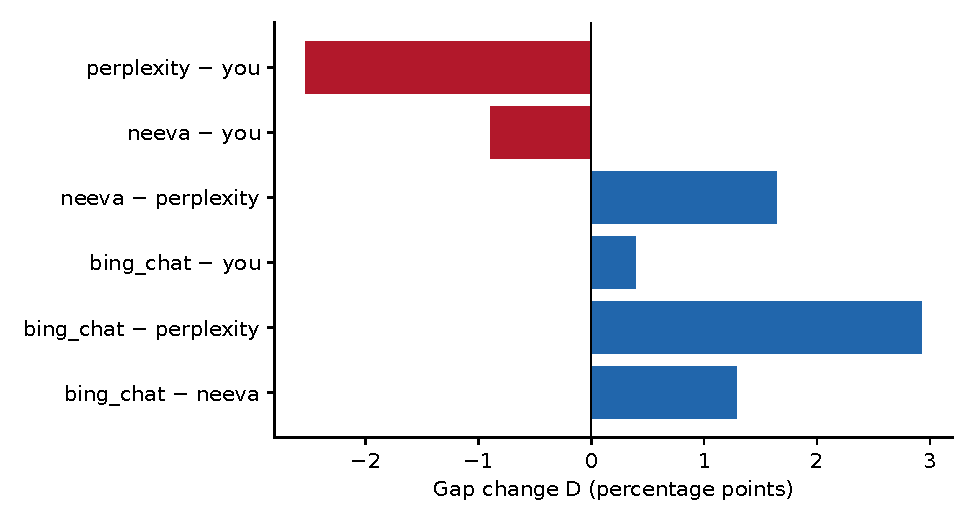
\includegraphics[width=\linewidth]{figures/gap_changes.pdf}
\caption{Primary gap changes. Positive values increase the signed advantage of the first system; negative values decrease it.}\Description{Horizontal bar chart showing six pairwise precision-gap changes. Four changes are positive and two are negative; the largest absolute change is 2.927 percentage points for Bing Chat versus Perplexity.}\label{fig:gaps}
\end{figure}
\section{Sensitivity and Failure Analysis}
\begin{table}[!htbp]\centering\small
\caption{Duplicate-handling sensitivity. System columns report mean precision loss in percentage points. Cohorts differ; this is not an isolated fixed-cohort annotation effect.}
\begin{tabular}{lrrrrr}\toprule
Variant & Queries & Bing Chat & Neeva & Perplexity & You\\\midrule
Primary & 353 & 0.826 & 2.111 & 3.753 & 1.220 \\
Identical collapse & 363 & 0.803 & 2.466 & 3.870 & 1.462 \\
Distinct mean & 369 & 0.790 & 2.426 & 3.915 & 1.573 \\
\bottomrule

\end{tabular}\label{tab:robustness}
\end{table}
\subsection{Repeated records}
One is an alternative which folds similar records together, and removes groups that contain conflicting records. The latter is averaging within a response/query, but keeps a copy of each unique eligible record. Both of these must provide valid citation mapping and coverage across all systems. They keep up to 363 and 369 queries, respectively (Table~\ref{tab:robustness}). Both preserve ordering. In contrast to the primary analysis, which showed a gap of 2.927, the Bing Chat--Perplexity gap changes are 3.066 and 3.125 points respectively. Record-resolution and cohort-expansion effects account for the differences.

\subsection{Pooled citations}
The citation of the main group as a whole gives greater value to the more cited answers. The gap changes between the Bing Chat and Perplexity is 2.996 points and the gap changes between Perplexity and You is $-1.872$ points. All orderings that were preserved in pairs are preserved.

\subsection{Mapping and label failures}
Conditional rows are identified for the 345 rows with non-bijective correspondence, for the 335 rows with unequal row counts, and for the 12 rows where the exact statement spans aren't found, or are not unique. These categories overlap. Since the protocol does not stipulate a minimum number of citations, none of the 892 rows of zero citations have specific precision. A total of 324 archival individual labels for support-plus-refutation collective judgments and 139 for accessible collective judgments, and 33 labels that are unclear to 9075 labels without collective judgments, also exist in the archive. The last 3 categories earn no credit and are able to be differentiated during the audit. An ineligible answer may cause all of the query to drop out of the common cohort, for example if the other systems made otherwise usable answers eligible.

\begin{figure}[!htbp]\centering
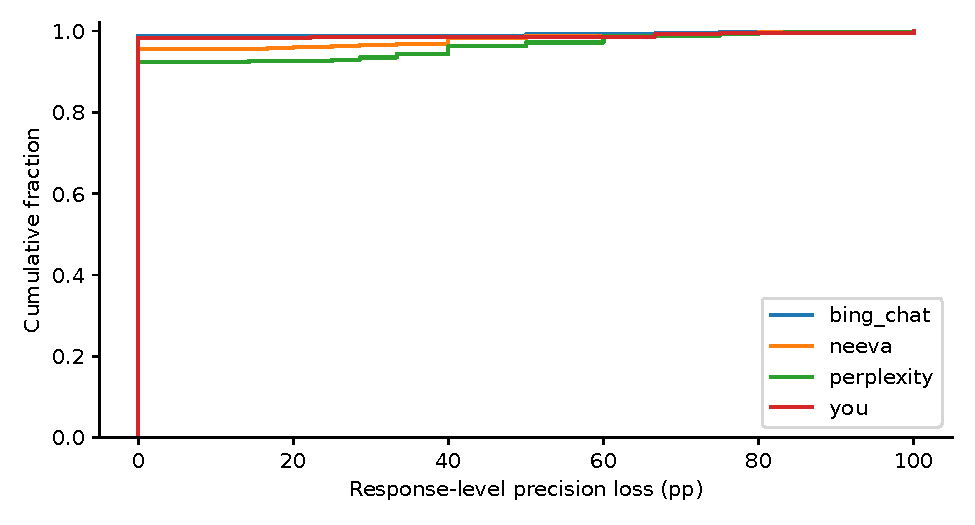
\includegraphics[width=\linewidth]{figures/loss_ecdf.pdf}
\caption{Response-level loss distribution. All four medians are zero; positive loss is confined to a small subset.}\Description{Empirical cumulative distribution curves for response-level precision loss across Bing Chat, Neeva, Perplexity, and You. All curves show a median loss of zero and a small tail of positive losses.}\label{fig:lossdist}
\end{figure}
\section{Discussion and Limitations}
\begin{figure}[!htbp]\centering
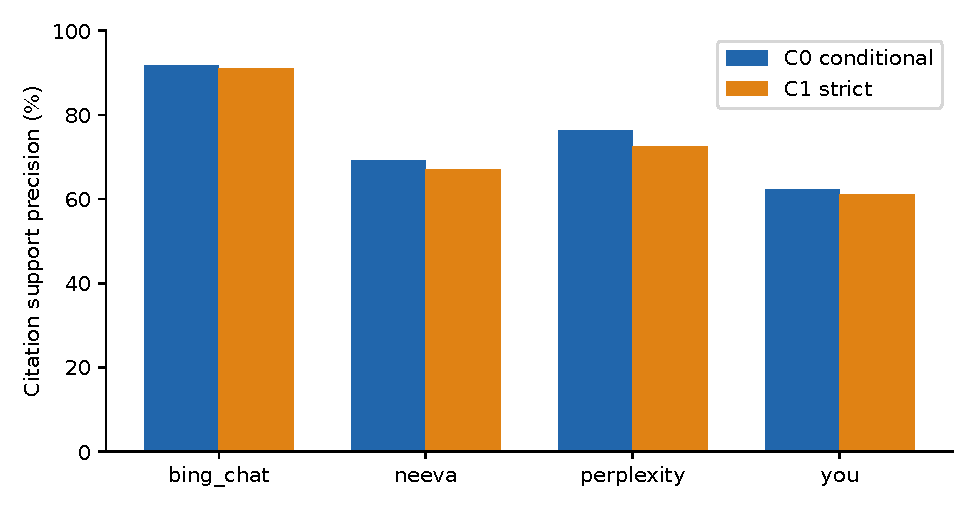
\includegraphics[width=\linewidth]{figures/precision.pdf}
\caption{Shared-cohort precision under both adapted controls. The chart starts at zero; differences are detailed in Table~\ref{tab:system}.}\Description{Grouped bar chart comparing C0 and C1 citation-support precision for Bing Chat, Neeva, Perplexity, and You. C1 is lower for all four systems.}\label{fig:precision}
\end{figure}
C0: payments are made for individual full support and for contributions that are part of collective evidence. In C1, individual sufficiency is measured. The C1 mathematical degradation is along the same lines, given that its credit rule is narrower. The empirical outcome is that the disparity in decline is sufficiently different between systems to shift gaps between the systems in either direction. These differences are interpretable when these units are reported in terms of the number of items in the citation, eligibility rules, and partial-credit rules, as well as in terms of the weight.

There should be unambiguous, cited answers from each of the systems for the chosen cohort. It may include additional elements of the archive in a different order and may have a different query. The historical response snapshot and inherited judgments restrict applicability of the concept to other query distributions, systems, and annotation protocols. These rules provide a separate type of citation support from source existence, metadata accuracy, recall, answer factuality and utility. A definitive duplication of the baseline and priority published remains unclarified for this exact reanalysis.

\section{Reproducibility and AI Accountability}
The submission contains the python pipeline, tests, protocol, auditable CSV/JSON output, figure generation, and LaTeX fragments of tables on results. The runner saves commands, exit status, input and code identity, environment and resource use. Writes to a new output directory. Not included in distributed evidence: raw response, source excerpts. Archive reuse terms apply and must be checked as these can vary.

AI support for source inspection, protocol/implementation development, tests, analysis, output checks, and drafting. An arithmetic audit will validate the manner in which scoring is applied to the archived labels. It does not make any stand-alone evidence judgements about human aspects.

\section{Conclusion}
For 353 frequent queries, adjustments to credit for partial citation support for only the two measures of precision (pairwise and in terms of precision-discounted error rate) change by as much as 2.927 percentage points, without altering order. Most of the answers came in relatively small clusters indicating losses. The tested conditions also maintained ordering for duplicate-handling alternatives and pooled-citation aggregation. The margins noted depend on the announced scoring policy.
\clearpage
\bibliographystyle{ACM-Reference-Format}
\bibliography{references}
\end{document}
